% Unofficial Technion - Israel Institute of Technology CS Poster Template
% Copied from UChicago version that is very popular :)
% v1.1.0 released September 8, 2022
% https://github.com/k4rtik/uchicago-poster
% a fork of https://github.com/anishathalye/gemini

\documentclass[final]{beamer}

% ====================
% Packages
% ====================

\usepackage[T1]{fontenc}
\usepackage{lmodern}
\usepackage[size=custom,width=120,height=72,scale=1.0]{beamerposter}
\usetheme{gemini}
\usecolortheme{technion}
\usepackage{graphicx, siunitx}
\usepackage{booktabs}
\usepackage{doi}
\usepackage[numbers]{natbib}
\usepackage[patch=none]{microtype}
\usepackage{tikz}
\usepackage{pgfplots}
\pgfplotsset{compat=1.18}
\usepackage{anyfontsize}

\pdfstringdefDisableCommands{%
\def\translate#1{#1}%
}

% ====================
% Lengths
% ====================

% If you have N columns, choose \sepwidth and \colwidth such that
% (N+1)*\sepwidth + N*\colwidth = \paperwidth
\newlength{\sepwidth}
\newlength{\colwidth}
\setlength{\sepwidth}{0.025\paperwidth}
\setlength{\colwidth}{0.3\paperwidth}

\newcommand{\separatorcolumn}{\begin{column}{\sepwidth}\end{column}}

% ====================
% Title
% ====================

\title{Uncertainty-Aware Deep Learning for Antimalarial Drug Discovery: \\ Robust VAE Models and Consensus Validation}

\author{Myke Vital SAO TEMGOUA$^{1}$, Jean-Pierre TCHAPET NJAFA$^{1}$, Penabei SAMAFOU$^{2}$, \\ Wilfred Fon MBACHAM$^{3}$, Serge Guy NANA ENGO$^{1}$}

\institute[shortinst]{$^{1}$Dept. of Physics, Univ. Yaoundé I, Cameroon \quad $^{2}$Univ. de Sherbrooke, Canada \quad $^{3}$Dept. of Biochemistry, Univ. Yaoundé I}

% ====================
% Footer (optional)
% ====================

\footercontent{
  \href{https://indico.ictp.it/event/10849}{ICTP Advanced School in Applied Machine Learning (smr 4228)} \hfill
  \textbf{23-31 July 2026 — Trieste, Italy} \hfill
  \href{mailto:myke-vital.sao@facsciences-uy1.cm}{myke-vital.sao@facsciences-uy1.cm}}

% ====================
% Logo (optional)
% ====================

% use this to include logos on the left and/or right side of the header:
% \logoright{\includegraphics[height=7cm]{logos/TCML_QR_CODE.eps}}
% \logoright{\includegraphics[height=7cm]{logos/cs-logo-white.png}}

% ====================
% Body
% ====================

% TRIM RULES: l b r t
\begin{document}
\addtobeamertemplate{headline}{}
{
    \begin{tikzpicture}[remember picture,overlay]
      \node [anchor=north west, inner sep=3cm] at ([xshift=0.0cm,yshift=1.0cm]current page.north west)
      {\includegraphics[scale=0.69,clip]{logos/uy1_logo.eps}}; % also try shield-white.eps
      \node [anchor=north east, inner sep=3cm] at ([xshift=0.0cm,yshift=1.5cm]current page.north east)
      {\includegraphics[scale=0.45,clip]{logos/ictp_logo.eps}};
      % \node [anchor=north west, inner sep=3cm] at ([xshift=0.0cm,yshift=2.5cm]current page.north west)
    \end{tikzpicture}
}

\begin{frame}[t]
\begin{columns}[t]
\separatorcolumn

\begin{column}{\colwidth}

  \begin{alertblock}{The Challenge}

  \textbf{247M malaria cases, 619K deaths (2023).} Rising resistance demands new drugs. \textbf{BUT:} Screening costs $>$1000 CPU-hrs/target—excluding endemic regions (94\% of cases).

  \vspace{0.3em}
  \textbf{Goal:} Systematic computational discovery of synthesizable antimalarial leads from African natural product chemical space. Target: validated screening protocol that enables resource-limited endemic institutions to identify multi-target drug candidates with favorable ADMET profiles.

  \vspace{0.3em}
  \textbf{Barriers:} (1) African NP databases remain computationally unexplored for scaffold-hopping beyond local neighborhood interpolation. (2) Single-method docking yields near-random enrichment (DEKOIS AUC 0.450). (3) Conventional approaches demand prohibitive computational costs where 94\% of malaria cases occur.

  \end{alertblock}

  \begin{block}{Solution: 99.3\% Cost Reduction}

  \textbf{Innovation:} VAE clustering + dual consensus (Vina+DiffDock) + MPO

  396 African NPs + 454 antimalarials → \textbf{65,856 hybrids} → 484 centroids (0.7\%)

  \begin{center}
    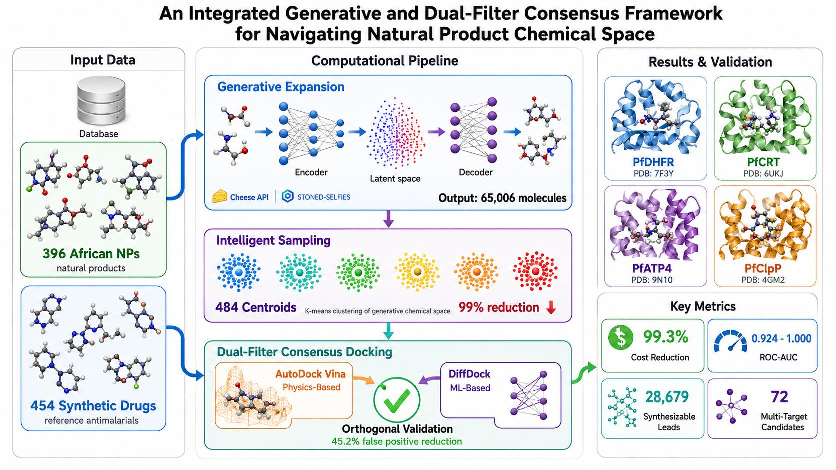
\includegraphics[width=0.7\linewidth]{images/graphical_abstract_final.pdf}
  \end{center}

  \textbf{Validation:} DEKOIS (AUC 0.450, Vina) → MMV Box (AUC 0.924--1.000, consensus, 69.8\% recovery)

  \textbf{Output:} \textbf{19,913 synthesizable leads} (4 \textit{P. falciparum} targets)

  \end{block}

  \begin{block}{VAE: Uncertainty via KL Divergence}

  \begin{minipage}{0.44\linewidth}
    \centering
    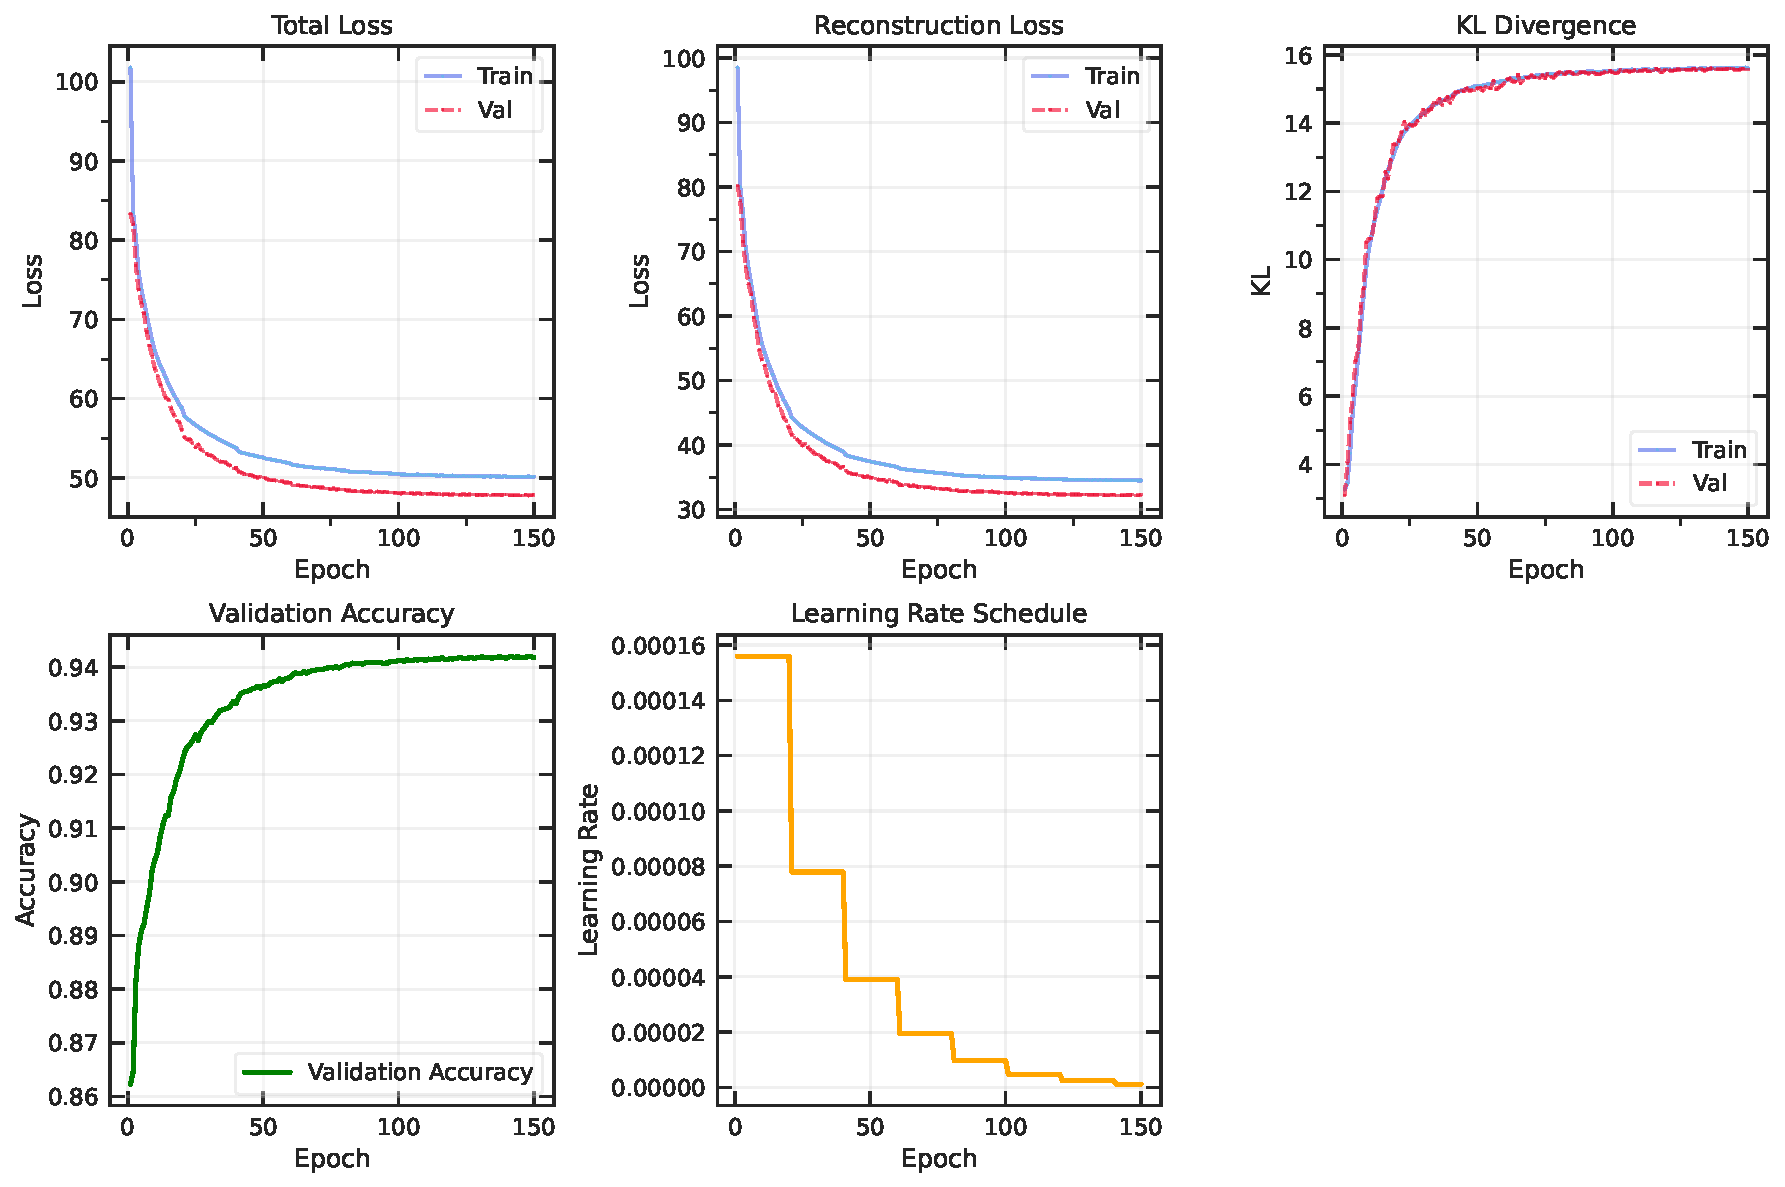
\includegraphics[width=\linewidth]{images/32_smi_vae_training_history_full.pdf}
    
    32D: 92.15\%, KL 6.43
  \end{minipage}
  \hfill
  \begin{minipage}{0.44\linewidth}
    \centering
    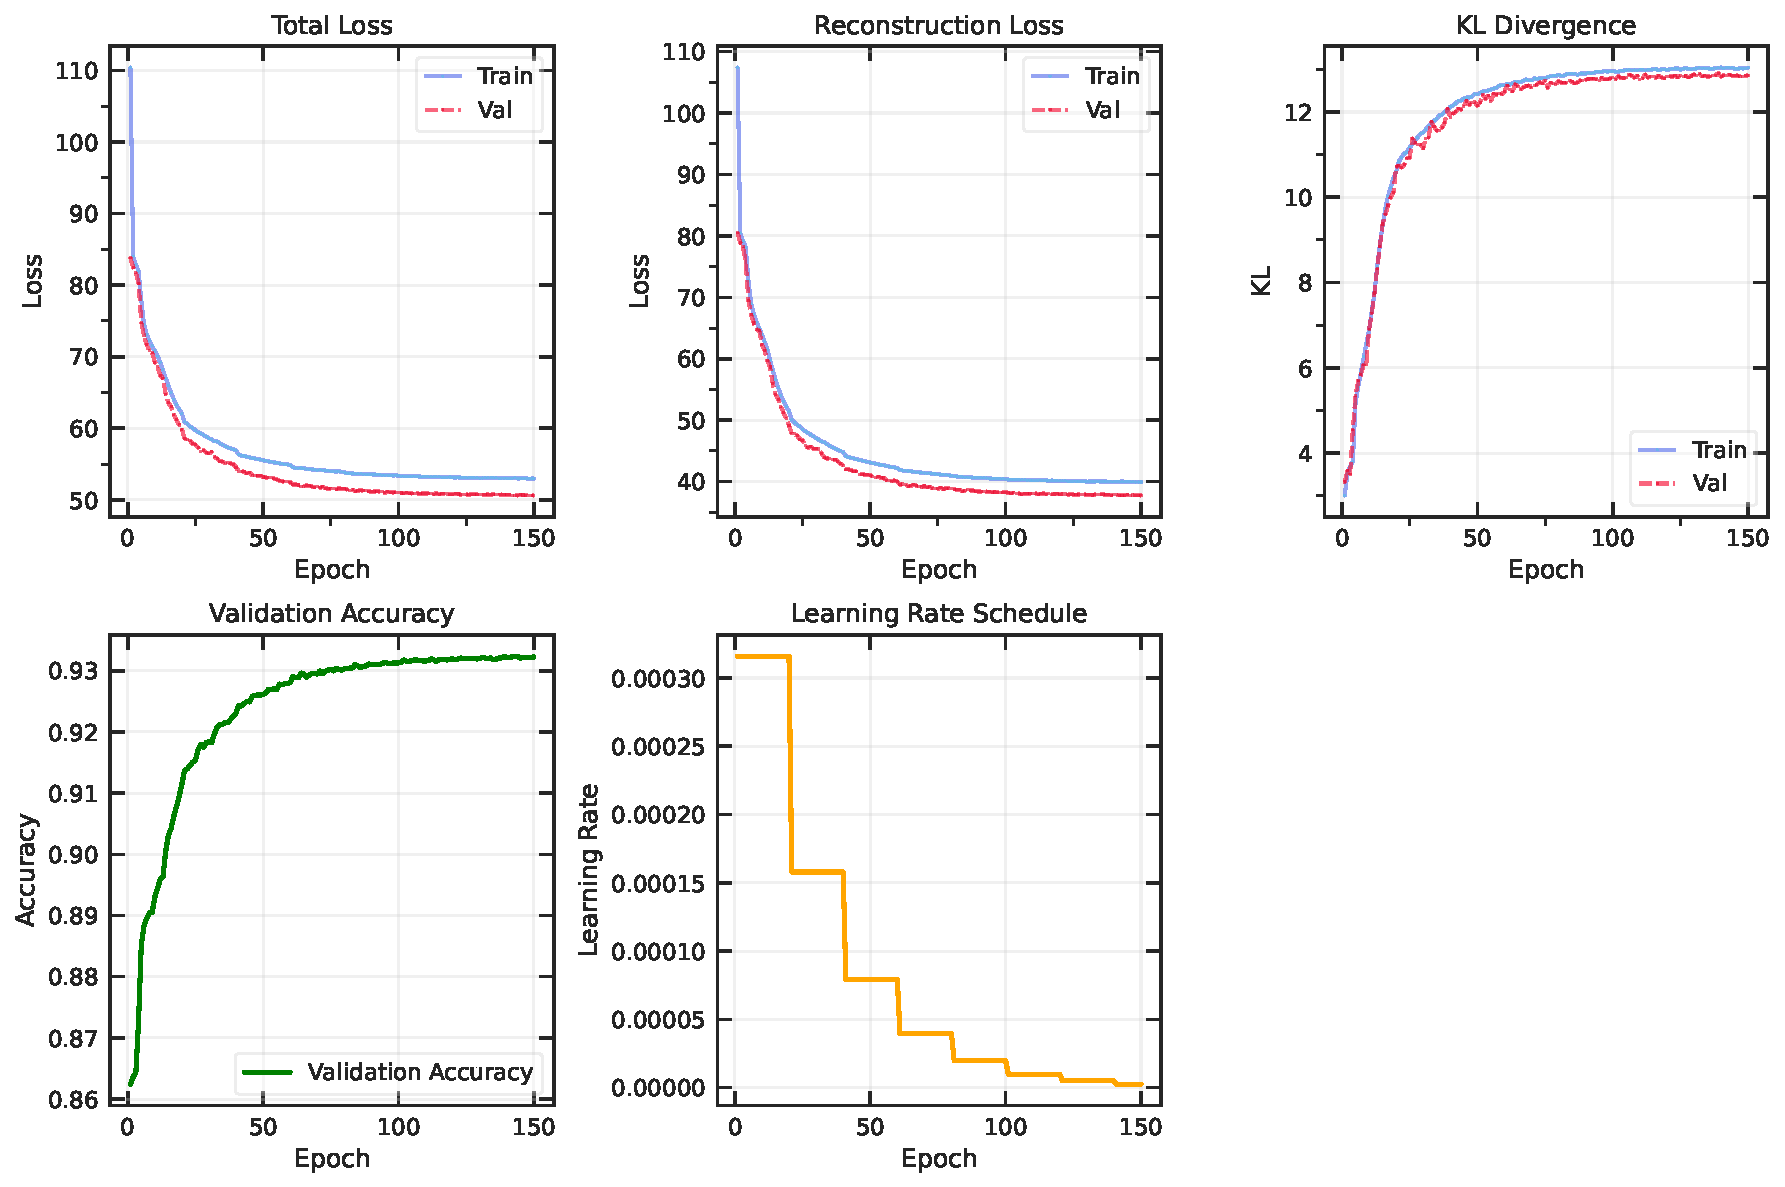
\includegraphics[width=\linewidth]{images/64_smi_vae_training_history_full.pdf}
    
    64D: 93.23\%, KL 12.86 ✓
  \end{minipage}

  \vspace{0.3em}
  \textbf{Why 64D?} Higher KL ($\uparrow$2$\times$) = explicit uncertainty—distinguishes confident from unreliable predictions.

  \textbf{Diversity:} 92.6\% novel + 69.3\% scaffold recovery = preserves cores, diversifies substituents.

  \end{block}

\end{column}

\separatorcolumn

\begin{column}{\colwidth}
	
\begin{block}{Clustering Quality}
	
	\begin{minipage}{0.48\linewidth}
		\centering
		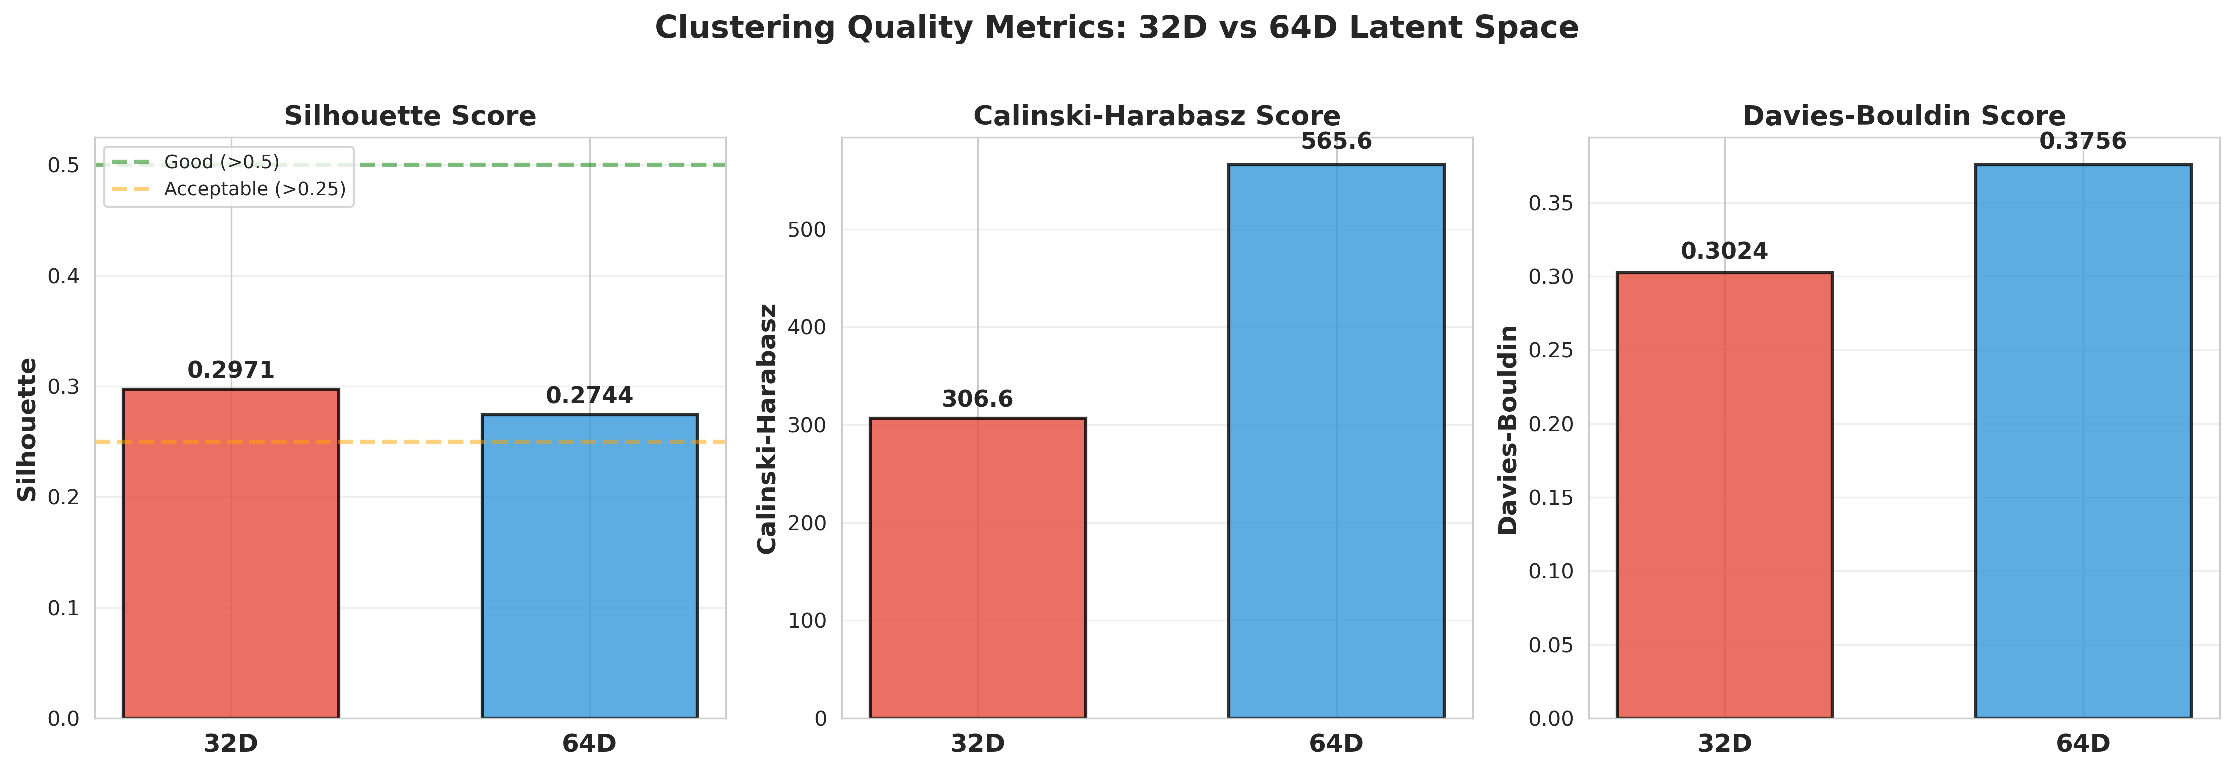
\includegraphics[width=\linewidth]{images/clustering_quality_comparison.pdf}
	\end{minipage}
	\hfill
	\begin{minipage}{0.48\linewidth}
		\centering
		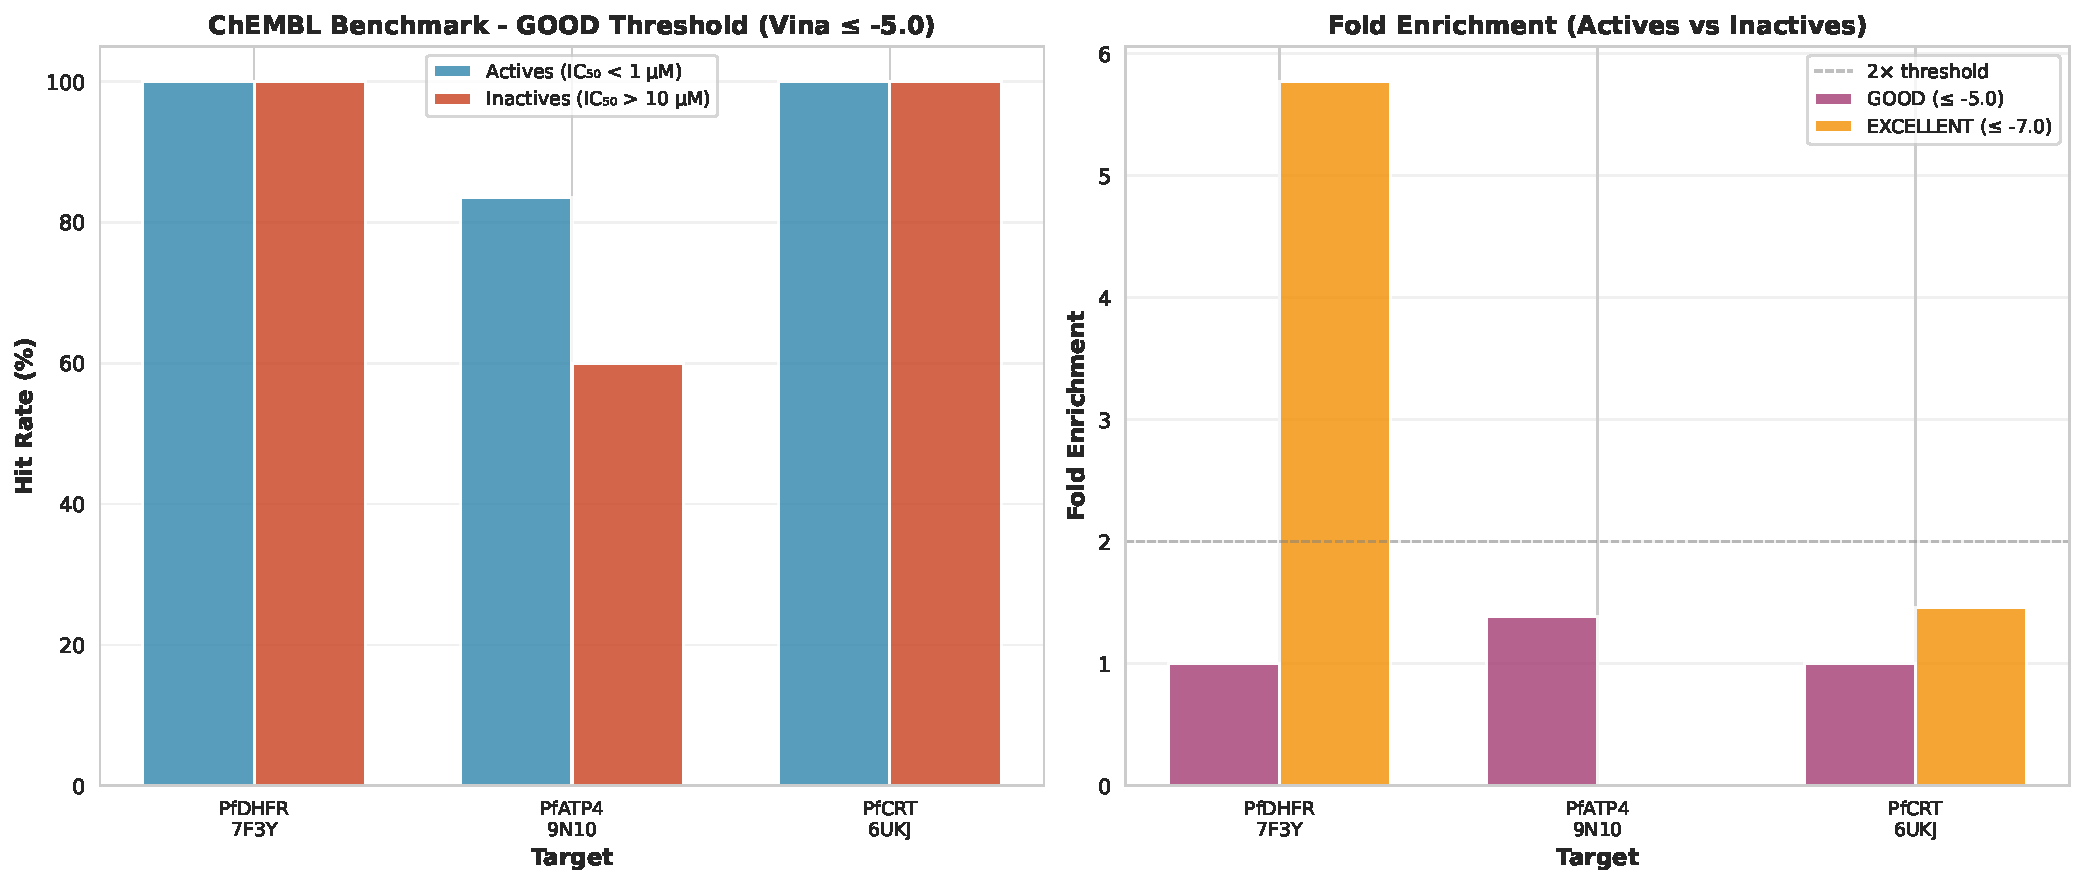
\includegraphics[width=\linewidth]{images/chembl_benchmark_comparison.pdf}
	\end{minipage}
	
	\vspace{0.3em}
	\textbf{KMeans:} Silhouette 0.23, CH 47.6, DB 2.45. \textbf{Intra Tanimoto 0.227 vs inter 0.101}—2$\times$ coherence.
	
\end{block}

\begin{block}{Dual Consensus Reduces False Positives}
	
	\begin{minipage}{0.51\linewidth}
		\centering
		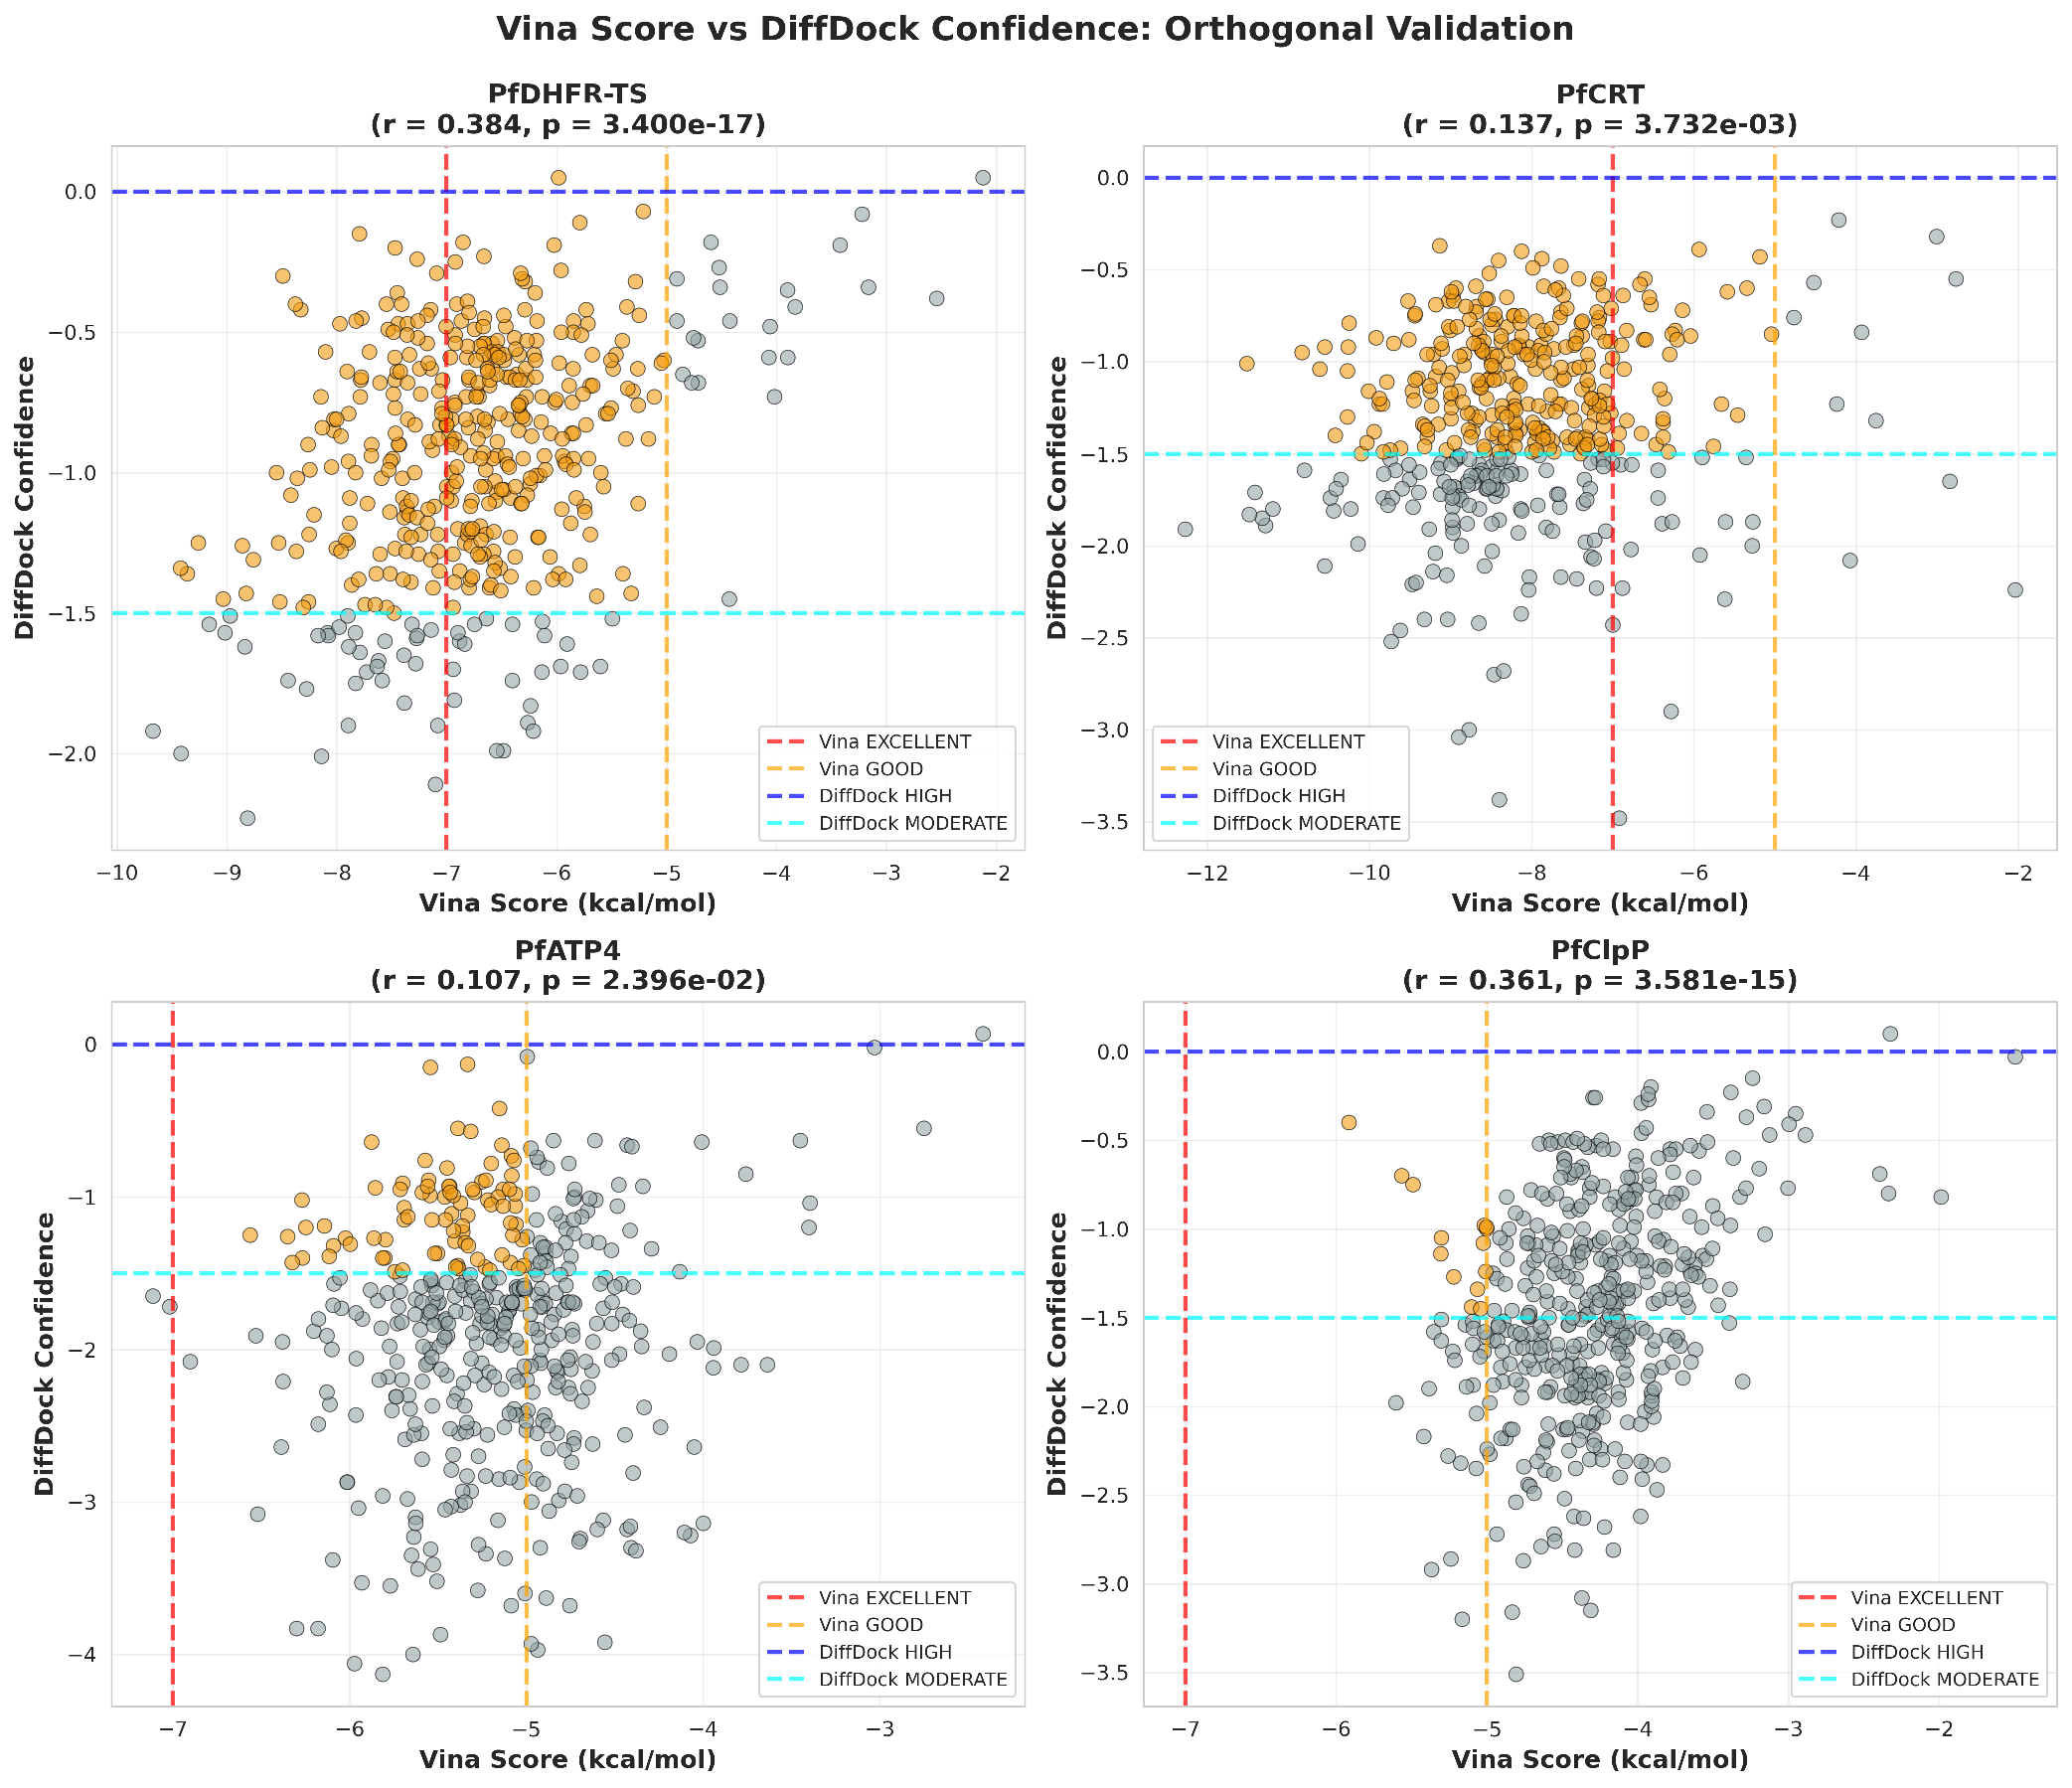
\includegraphics[width=\linewidth]{images/consensus_correlation_analysis.pdf}
	\end{minipage}
	\hfill
	\begin{minipage}{0.51\linewidth}
		\centering
		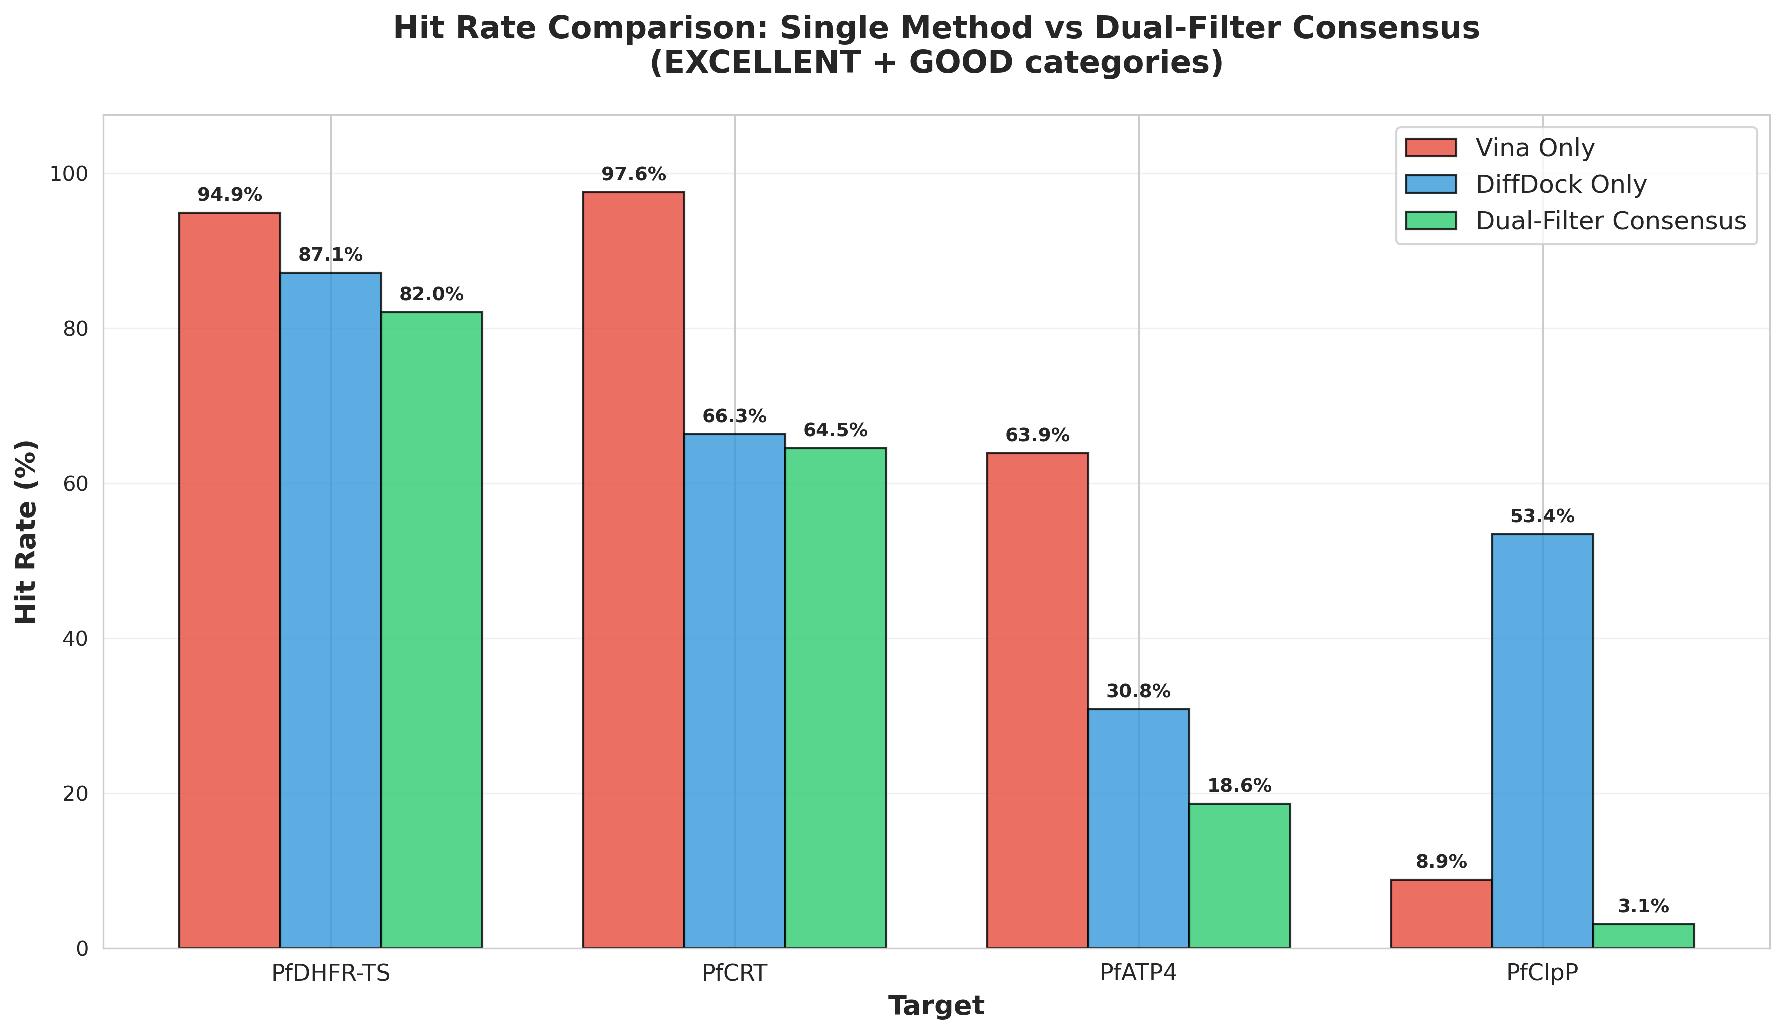
\includegraphics[width=\linewidth]{images/consensus_hit_rate_comparison.pdf}
	\end{minipage}
	
	\vspace{0.3em}
	\textbf{Why consensus?} DEKOIS: Vina-only AUC 0.450 (near-random). Vina $\perp$ DiffDock (r=0.1--0.4) = complementary.
	
	\textbf{Impact:} 12--45\% FP reduction. MMV: 69.8\% recovery, AUC 0.924--1.000.
	
\end{block}
	
\begin{block}{Rigorous Benchmarking}
	
	\begin{minipage}{0.48\linewidth}
		\centering
		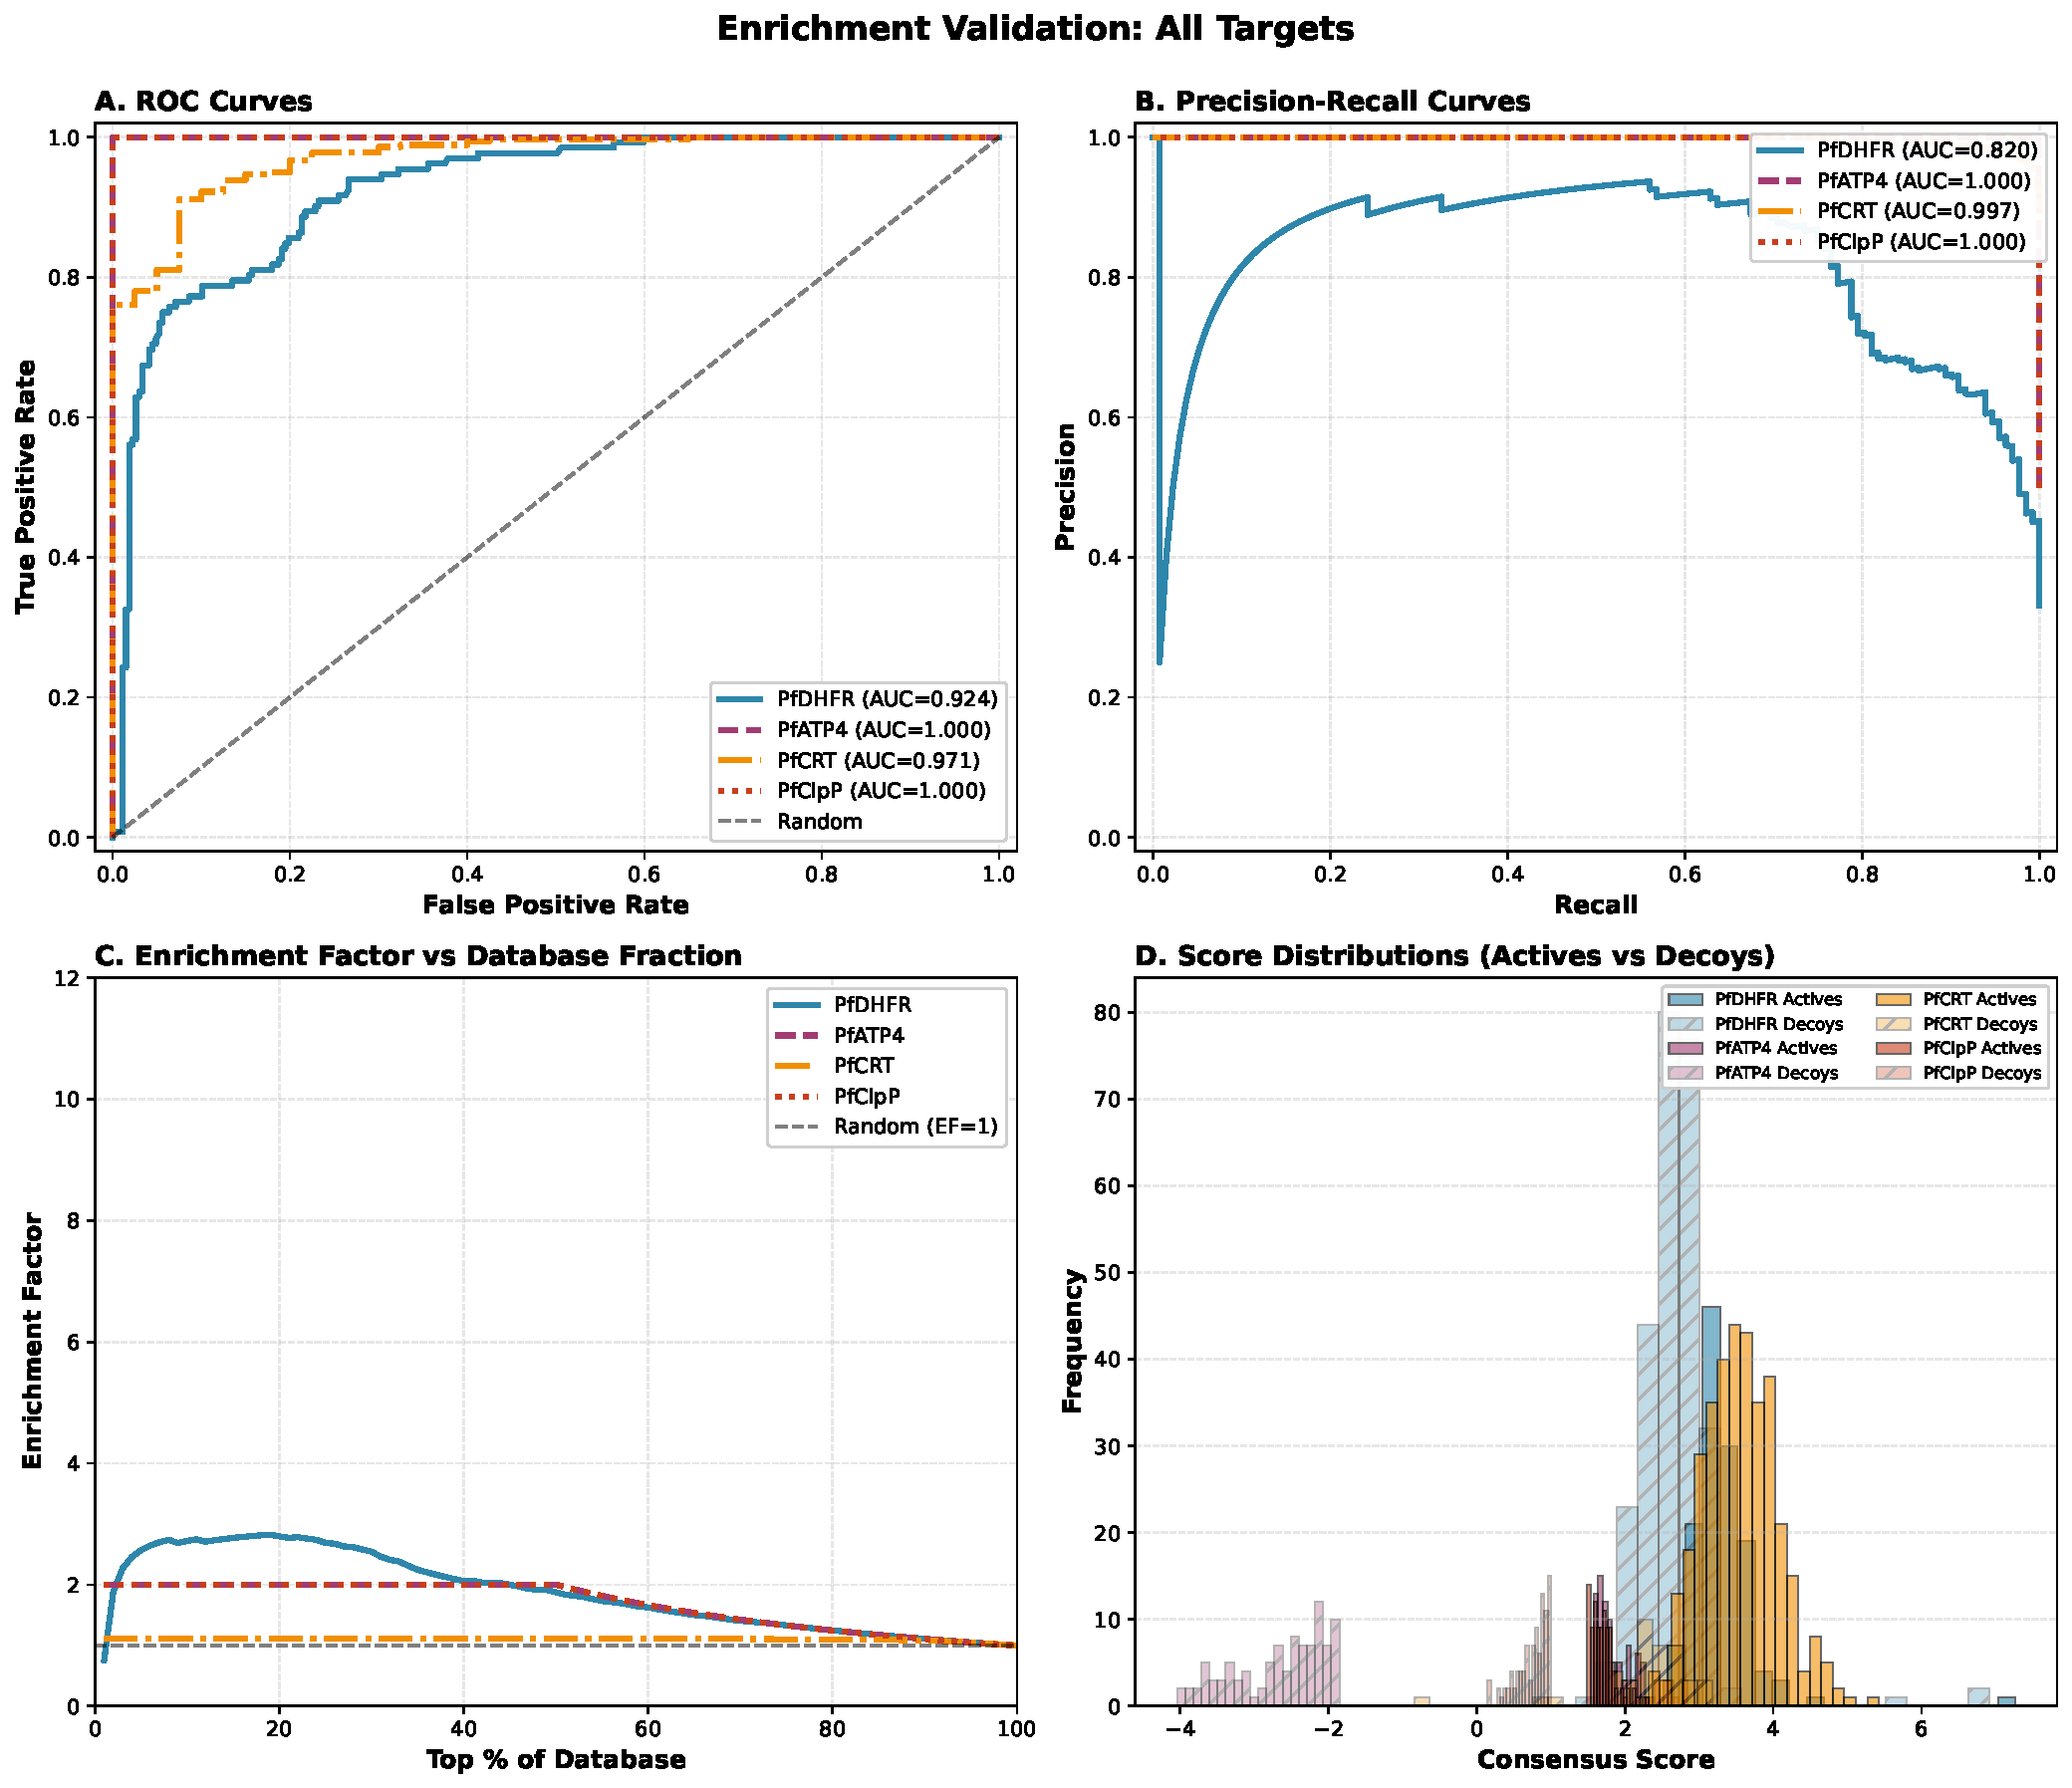
\includegraphics[width=\linewidth]{images/enrichment_all_targets_combined.pdf}
	\end{minipage}
	\hfill
	\begin{minipage}{0.48\linewidth}
		\centering
		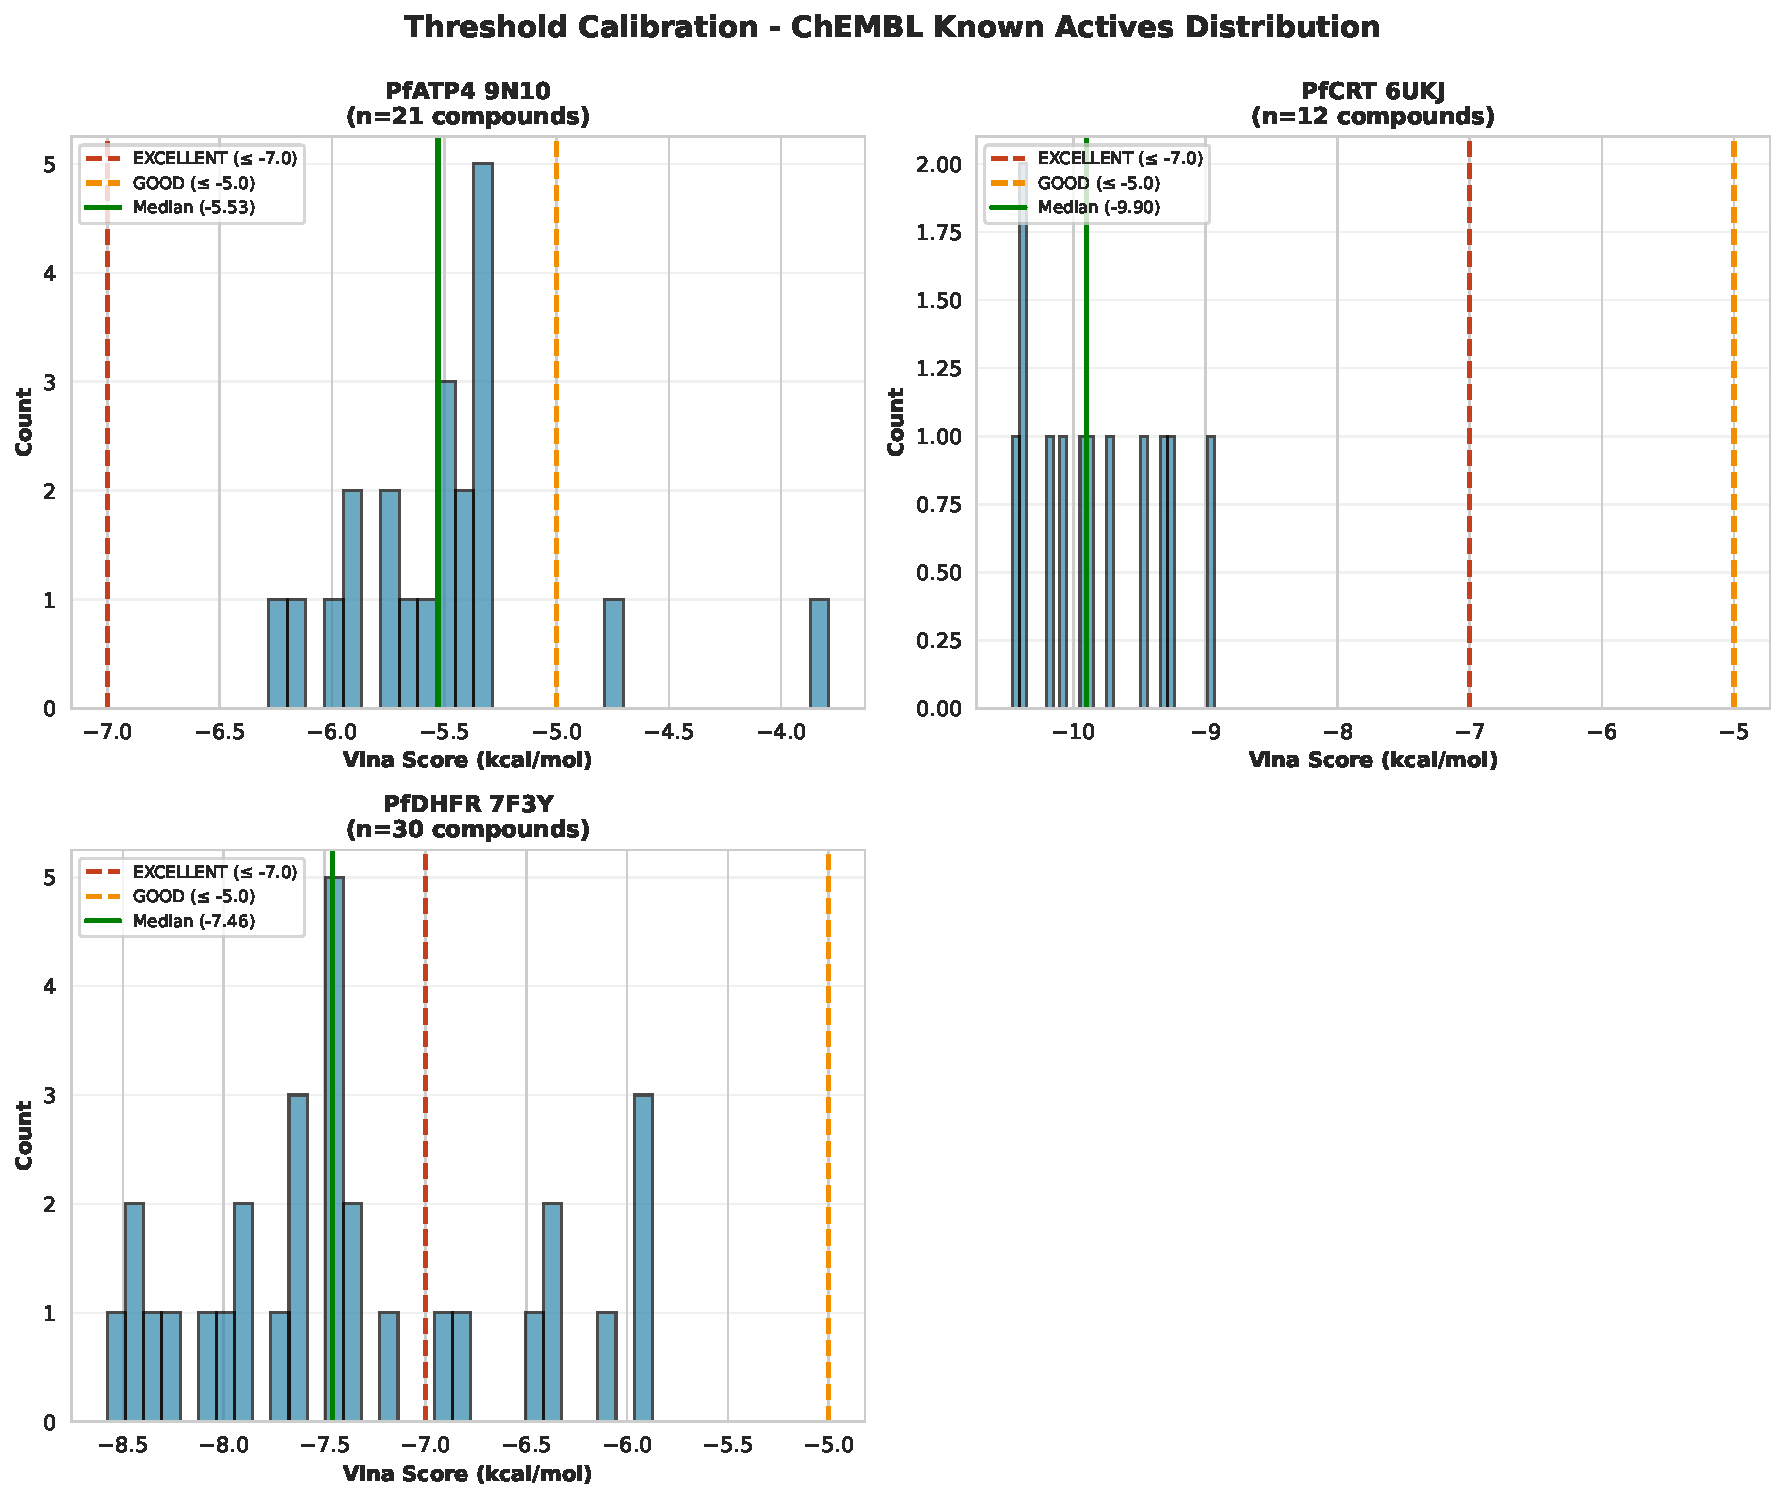
\includegraphics[width=\linewidth]{images/threshold_calibration_distribution.pdf}
	\end{minipage}
	\vspace{0.3em}
	
	\textbf{Prospective:} DEKOIS 40 actives + 1200 decoys, Vina AUC 0.450.
	
	\textbf{Retrodictive:} MMV 399 antimalarials, consensus AUC 0.924--1.000 (bootstrap 95\% CI). Top 5\% enrichment.
	
	\textbf{Thresholds:} ChEMBL −6.9 → EXCELLENT $\leq$−7.0, GOOD −7.0 to −5.0.
\end{block}
  
\end{column}

\separatorcolumn

\begin{column}{\colwidth}

  \begin{block}{Results: Drug-Like Multi-Target Leads}

  \begin{minipage}{0.48\linewidth}
    \centering
    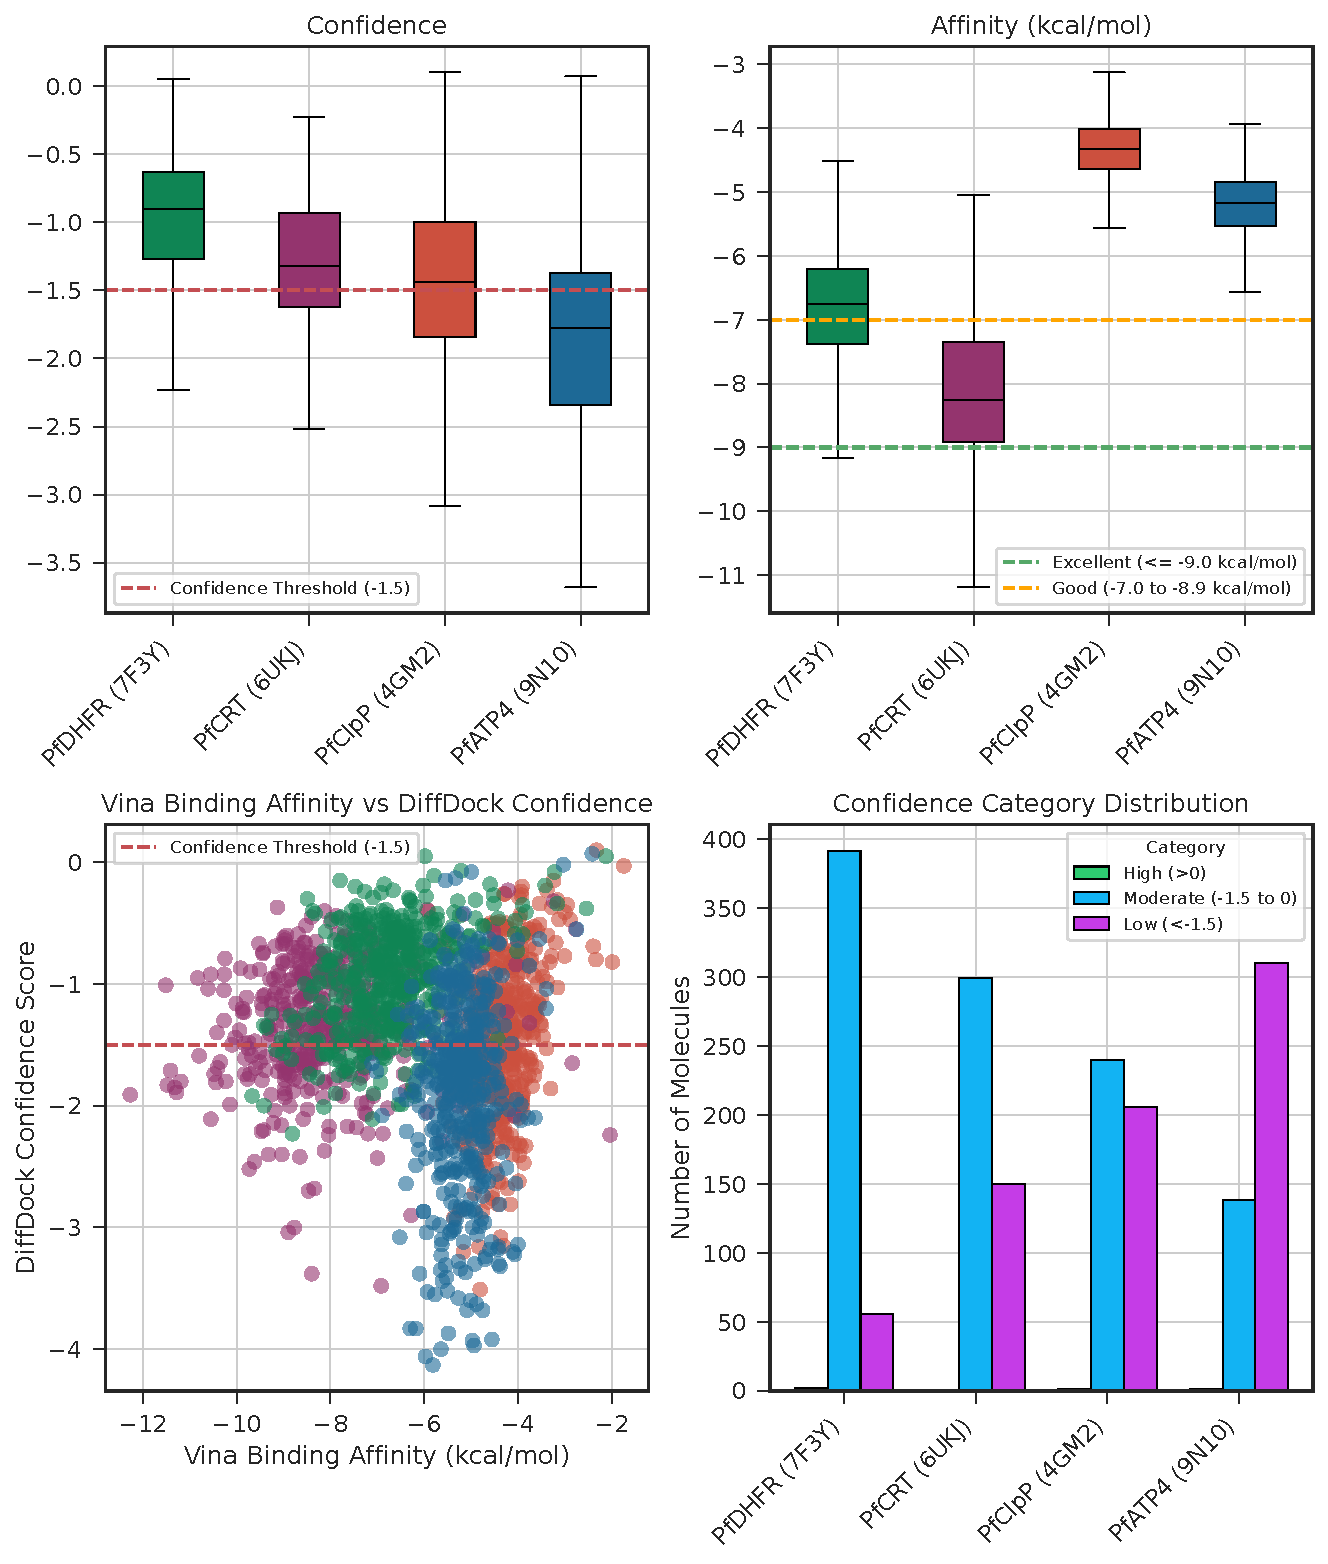
\includegraphics[width=\linewidth]{images/docking_summary_4panel.pdf}
  \end{minipage}
  \hfill
  \begin{minipage}{0.48\linewidth}
    \centering
    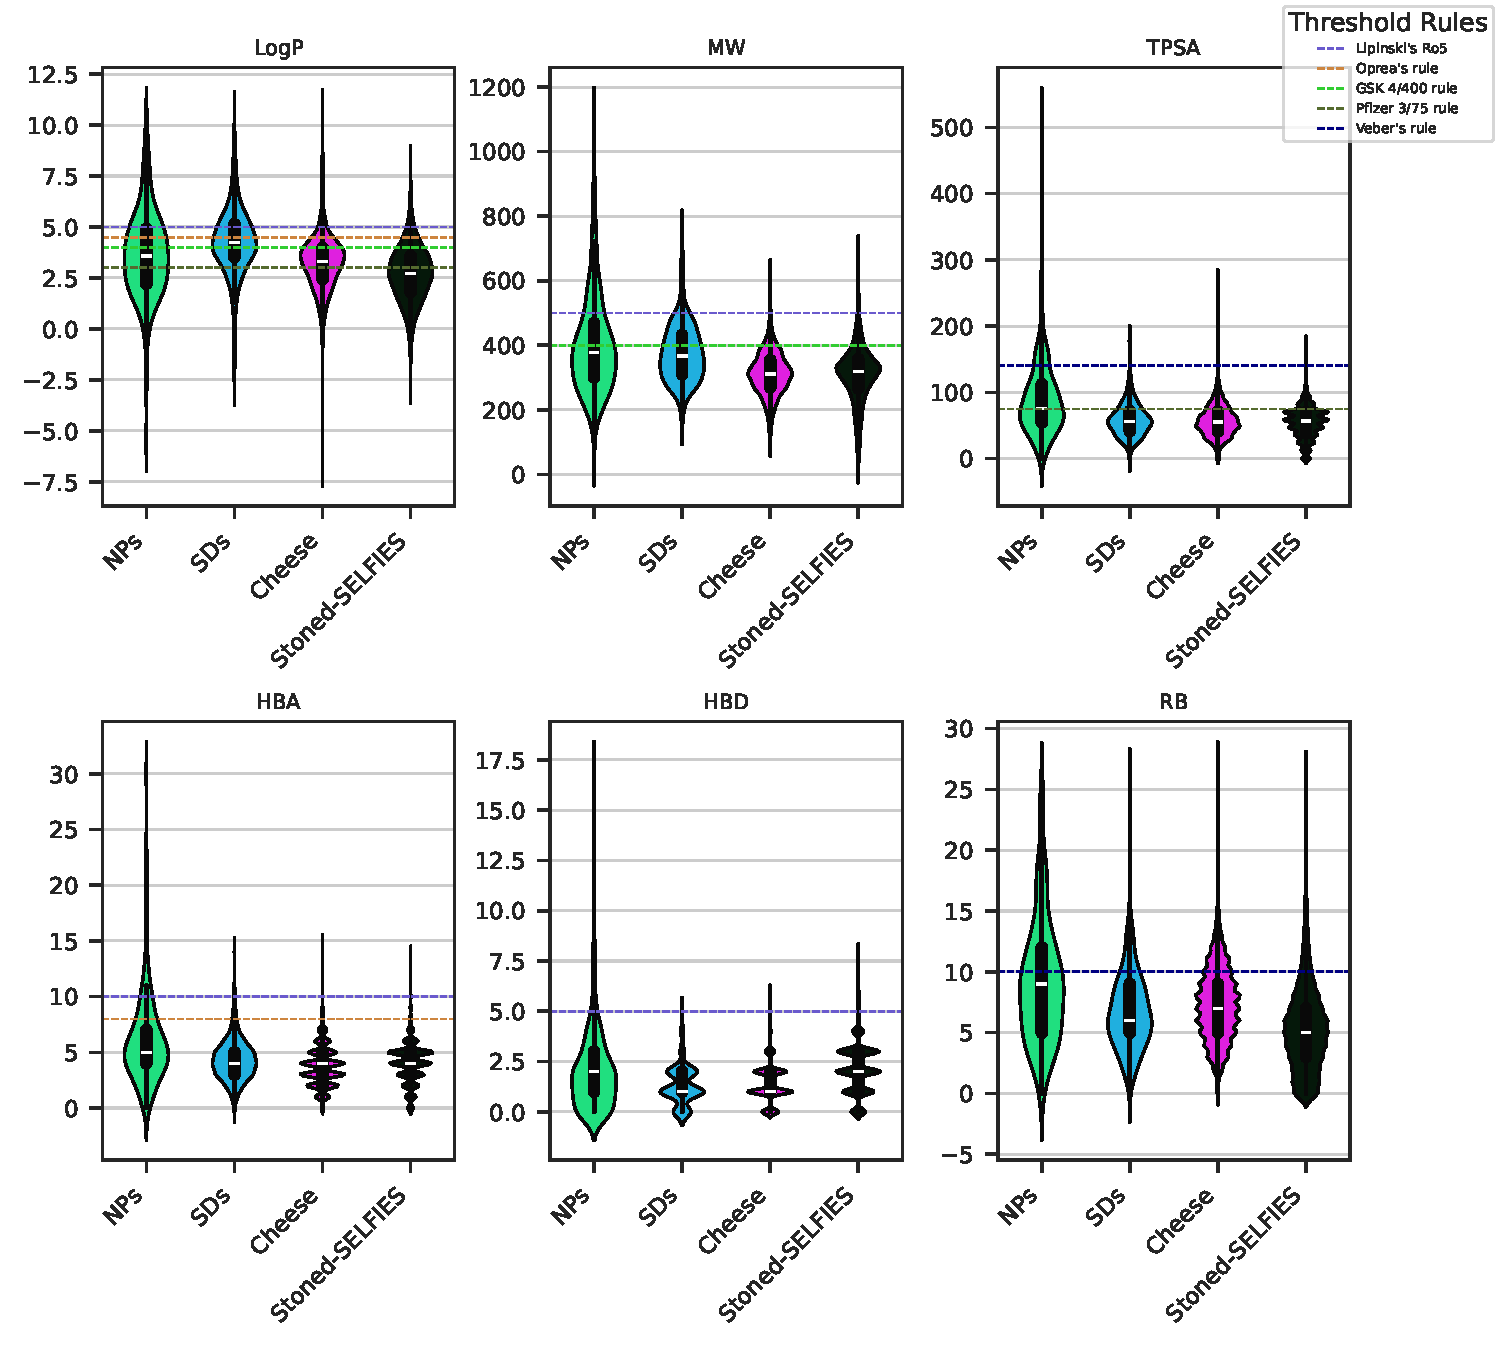
\includegraphics[width=\linewidth]{images/phys_chem.pdf}
  \end{minipage}

  \vspace{0.3em}
  \textbf{Targets:} PfDHFR, PfCRT, PfClpP, PfATP4. Consensus $<$−8 kcal/mol.
  
  \textbf{Drug-like:} 94.1\% Lipinski, 88.5\% Veber, 57\% synthesizable.
  
  \textbf{Multi-target:} $>$70 candidates. \textbf{100\% SI$>$10} (810 seeds).

  \end{block}

  \begin{alertblock}{Key Achievements}

  \textbf{19,913 leads} $\bullet$ \textbf{99.3\%} cost ↓ $\bullet$ \textbf{12--45\%} FP ↓ $\bullet$ \textbf{AUC 0.924--1.000} $\bullet$ \textbf{$>$70 multi-target} $\bullet$ \textbf{100\% SI$>$10}

  \end{alertblock}

  \begin{block}{Impact \& Open Science}

  \small
  \textbf{Innovation:} VAE KL ($\uparrow$2$\times$) = uncertainty $\bullet$ Dual consensus = 12--45\% FP ↓ $\bullet$ Dual benchmarking = pharma reliability

  \textbf{Practical:} Endemic access—$>$1000 → $<$10 CPU-hrs/target (94\% cases)

  \textbf{Open:} Zenodo 10.5281/zenodo.19608875

  \vspace{0.4em}
  \textbf{Conclusion:} This framework democratizes antimalarial discovery by enabling comprehensive multi-target screening in malaria-endemic research institutions where computational resources are limited but scientific need is greatest. By combining rigorous validation (MMV Box AUC 0.924--1.000) with 99.3\% cost reduction, we establish a reproducible pathway from African biodiversity to synthesizable drug candidates—transforming regional computational barriers into opportunities for locally-driven pharmaceutical innovation.

  \end{block}

  \begin{block}{References}

    \nocite{*}
    \scriptsize{\bibliographystyle{plain}\bibliography{poster}}

  \end{block}

\end{column}

\separatorcolumn
\end{columns}
\end{frame}

\end{document}
